\documentclass[conference]{IEEEtran}
\usepackage{times}

% numbers option provides compact numerical references in the text.
\usepackage[numbers]{natbib}
\usepackage{multicol}
\usepackage[bookmarks=true]{hyperref}
\usepackage{amssymb}
\usepackage{amsmath}
\usepackage{booktabs}
\usepackage{graphicx}
\usepackage{tikz}
\usetikzlibrary{positioning,arrows.meta}

\pdfinfo{
   /Author (Kangwei Sun)
   /Title  (EmoMoconvq: Emotion-Conditioned Human Motion Generation -- Midterm Report)
   /Subject (Physics-based motion generation)
   /Keywords (motion generation; emotion conditioning; physics-based)
}

\begin{document}

\title{EmoMoconvq: Emotion-Conditioned Human Motion Generation\\[3pt]
\large Midterm Progress Report}

\author{Kangwei Sun 524531910006}

\maketitle

\begin{abstract}
Physics-based motion generation methods such as MoConVQ~\cite{yao2023moconvq}
produce high-quality motions from text but generate stylistically neutral
results regardless of emotional context. This project, \textbf{EmoMoconvq},
extends MoConVQ's text-to-motion transformer (T2M-MoConGPT) by injecting a
discrete emotion label as an additional conditioning signal, learned through
parameter-efficient fine-tuning. As a method-extension project, we build
directly on the pretrained MoConVQ framework and add a trainable emotion
module without modifying the original code. This report summarizes concrete
progress: (i)~the T2M-MoConGPT baseline has been reproduced and verified;
(ii)~an emotion-labelled text corpus has been curated from
HumanML3D~\cite{guo2022generating} by keyword filtering; (iii)~the emotion
embedding module has been implemented and verified to be a clean parameter
superset of the pretrained checkpoint; and (iv)~a from-scratch negative
log-likelihood fine-tuning loop has been implemented and validated in a
controlled experiment, where the loss decreases from $6.95$ to $\sim\!10^{-4}$
and the emotion module receives non-zero gradients throughout. We also report
honest preliminary findings -- a smaller-than-expected labelled set and a
representation gap in the motion-tokenization pipeline -- and how they shape
the remaining plan.
\end{abstract}

\IEEEpeerreviewmaketitle

\section{Problem Statement and Motivation}
Human motion is inherently expressive: the same action performed in different
emotional states (e.g., walking while happy vs.\ sad) exhibits distinct
kinematic patterns such as stride length, torso posture, and arm-swing
amplitude. This expressiveness is critical for digital humans, game
characters, and social robots, yet current physics-based generation methods
ignore it entirely.

MoConVQ~\cite{yao2023moconvq} shows that discrete residual-VQ representations
combined with a GPT-style transformer can generate diverse, physically
accurate motions from natural language. However, its T2M-MoConGPT produces
emotion-neutral outputs: the same text prompt always yields the same stylistic
result. The robot-learning problem we address is therefore \emph{how to
condition a pretrained generative motion model on a high-level affective
signal while preserving the physical plausibility guaranteed by its simulator}.
We address it with EmoMoconvq, which extends T2M-MoConGPT with discrete
emotion conditioning. The project scope is unchanged from the proposal; the
refinements below (a feature-dimension correction and a newly identified
data-pipeline gap) are implementation-level findings rather than a change of
direction.

\section{Related Work}
\textbf{Physics-based motion generation.}
MoConVQ~\cite{yao2023moconvq} encodes motions into residual VQ codes and
decodes them through a physics simulator via model-based RL, trained on 23
hours of motion data. Its frozen encoder and codebook make it well suited for
lightweight downstream fine-tuning, which is the basis of our work.

\textbf{Text-to-motion generation.}
T2M-GPT~\cite{zhang2023t2m} and MDM~\cite{tevet2022human} generate kinematic
motions from text using discrete transformers and diffusion models
respectively, both trained on HumanML3D~\cite{guo2022generating}. Neither is
physics-based nor models emotional style.

\textbf{Style and emotion in motion.}
ACTOR~\cite{petrovich2021action} conditions a Transformer VAE on action
labels, showing that categorical signals can guide motion style. The CMU MoCap
database~\cite{cmu_mocap} contains emotionally performed locomotion. Our work
is, to our knowledge, the first to combine emotion conditioning with a
physics-based generation pipeline. For parameter-efficient adaptation we draw
on the adapter/LoRA family~\cite{hu2022lora}.

\section{Technical Approach}

\subsection{System Overview}
We build on the pretrained MoConVQ framework~\cite{yao2023moconvq}, which has
three trained components: (1)~a 1D-convolutional \textbf{motion encoder}
$\mathcal{E}$ mapping a motion clip to latent vectors; (2)~a \textbf{residual
VQ codebook} $\mathcal{B}$ ($N=8$ quantization layers, 512 codes of dimension
768) producing discrete index sequences; and (3)~a \textbf{physics-based
decoder} $\mathcal{D}$ (deconvolution + mixture-of-experts policy + simulator).
For text-to-motion, MoConVQ uses a dual transformer \textbf{MoConGPT}: a
\emph{temporal transformer} ($N_T=12$ cross-attention layers) that aggregates
information across time, and a \emph{depth transformer} ($N_D=5$ layers) that
predicts the RVQ indices layer by layer within each time step. We freeze all
of these and introduce a trainable emotion module plus a small number of
top temporal-transformer layers.

\subsection{Emotion Embedding Module}
Let $\mathcal{C}=\{\textit{neutral},\textit{happy},\textit{sad},\textit{angry},
\textit{fearful}\}$, $|\mathcal{C}|=5$. Each emotion is mapped to a trainable
vector
\begin{equation}
  E_e:\mathcal{C}\rightarrow\mathbb{R}^{d_e},\qquad e_c=E_e(c),
\end{equation}
with $d_e=512$. It is fused with the text feature through a two-layer MLP and
element-wise addition:
\begin{equation}
  f_{\text{cond}} = f_{\text{T5}} + \text{MLP}_{\text{proj}}(e_c).
  \label{eq:fuse}
\end{equation}
\textbf{Dimension correction.} The proposal stated $d_e$ matches the temporal
transformer hidden size; on inspection, the feature consumed by the
cross-attention layers is the \emph{1024-dimensional} T5-large~\cite{raffel2020t5}
text feature $f_{\text{T5}}$. Hence $\text{MLP}_{\text{proj}}:\mathbb{R}^{512}
\!\rightarrow\!\mathbb{R}^{1024}$, and fusion occurs in the text-feature space,
immediately after the text encoder and before the temporal transformer's
cross-attention blocks. The fused $f_{\text{cond}}$ replaces $f_{\text{T5}}$ in
those layers, exactly the original injection mechanism.

\textbf{Graceful-degradation initialization.} The last layer of
$\text{MLP}_{\text{proj}}$ is zero-initialized, so at the start of fine-tuning
$\text{MLP}_{\text{proj}}(e_c)=\mathbf{0}$ and $f_{\text{cond}}=f_{\text{T5}}$:
the model is numerically identical to the pretrained baseline and can only
improve from there. This design is verified empirically in
Section~\ref{sec:exp}. Figure~\ref{fig:arch} summarizes the architecture.

\begin{figure*}[t]
\centering
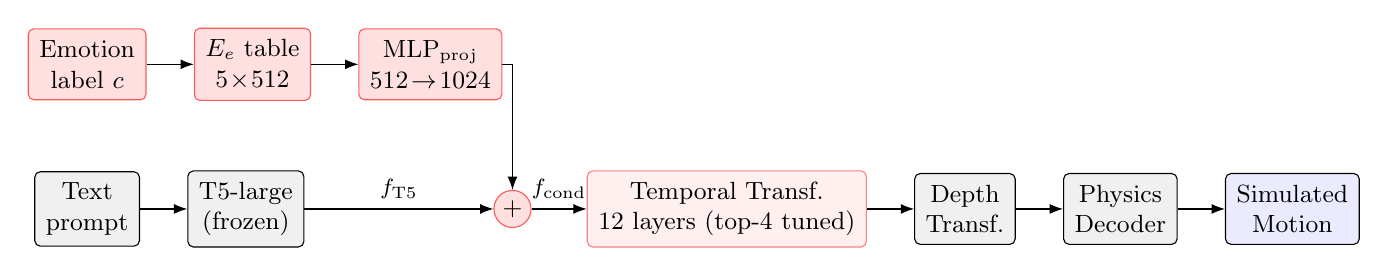
\begin{tikzpicture}[
  font=\small,
  box/.style={draw,rounded corners=2pt,minimum height=9mm,align=center,inner sep=4pt},
  frozen/.style={box,fill=gray!12},
  train/.style={box,fill=red!12,draw=red!65},
  op/.style={draw,circle,inner sep=1.4pt,fill=red!12,draw=red!65},
  >=Latex]
\node[train] (emo) {Emotion\\label $c$};
\node[train,right=6mm of emo] (Ee) {$E_e$ table\\$5\!\times\!512$};
\node[train,right=6mm of Ee] (mlp) {$\text{MLP}_{\text{proj}}$\\$512\!\to\!1024$};
\node[frozen,below=9mm of emo] (text) {Text\\prompt};
\node[frozen,right=6mm of text] (t5) {T5-large\\(frozen)};
\node[op,right=24mm of t5] (plus) {$+$};
\node[box,fill=red!6,draw=red!50,right=7mm of plus] (temp) {Temporal Transf.\\12 layers (top-4 tuned)};
\node[frozen,right=6mm of temp] (depth) {Depth\\Transf.};
\node[frozen,right=6mm of depth] (dec) {Physics\\Decoder};
\node[box,fill=blue!8,right=6mm of dec] (motion) {Simulated\\Motion};
\draw[->] (emo)--(Ee);
\draw[->] (Ee)--(mlp);
\draw[->] (text)--(t5);
\draw[->] (t5)-- node[above,font=\footnotesize]{$f_{\text{T5}}$} (plus);
\draw[->] (mlp.east) -| (plus.north);
\draw[->] (plus)-- node[above,font=\footnotesize]{$f_{\text{cond}}$} (temp);
\draw[->] (temp)--(depth);
\draw[->] (depth)--(dec);
\draw[->] (dec)--(motion);
\end{tikzpicture}
\caption{EmoMoconvq architecture. Red blocks are trainable (the emotion
module and the top-4 temporal-transformer layers); grey blocks are frozen
pretrained MoConVQ components. The emotion signal is injected additively into
the T5 text feature (Eq.~\ref{eq:fuse}).}
\label{fig:arch}
\end{figure*}

\subsection{Fine-Tuning Strategy}
We freeze the encoder, codebook, physics decoder, depth transformer, the text
encoder, and the bottom $(N_T-K)$ temporal-transformer layers. Only the
emotion table $E_e$, the projection $\text{MLP}_{\text{proj}}$, and the top
$K=4$ temporal layers are trained, with the same negative log-likelihood (NLL)
objective as MoConGPT:
\begin{equation}
  \mathcal{L}_{\text{emo}}=\mathbb{E}_{(S,c)}\!\left[\sum_{k}\sum_{d}
  -\log p\!\left(I^k_d \mid f_{\text{cond}}(c),\,I^k_{<d},\,I^{<k}\right)\right].
  \label{eq:nll}
\end{equation}
The official MoConVQ release does not include MoConGPT training code, so this
loop is implemented from scratch following the teacher-forcing structure of
the model. The emotion module is realized as a non-invasive subclass
(\texttt{EmoText2Motion\_Transformer}); the original MoConVQ source is left
unmodified, which keeps the baseline runnable for ablation and makes our
contribution explicit. Parameter counts are reported in
Table~\ref{tab:verify}.

\subsection{Data Preparation}
Following the proposal, we filter the HumanML3D~\cite{guo2022generating}
training split for captions containing emotion-related adverbs/adjectives
(e.g., ``happily'', ``sadly'', ``angrily'', ``fearfully''), grouped into four
non-neutral classes, and assign labels by keyword matching. Captions matching
two classes are treated as conflicts and discarded.

\section{Preliminary Experiments and Results}
\label{sec:exp}

\subsection{Baseline Reproduction}
The pretrained T2M-MoConGPT pipeline was installed and reproduced. From the
text prompt \textit{``A person walking while talking on the phone''} the system
generated a physically simulated motion of 840 frames at 120\,fps (7\,s).
Figure~\ref{fig:baseline} shows representative frames of the simulated
character, confirming the baseline produces plausible, physically valid
motion and that our environment is correct.

\begin{figure}[t]
\centering
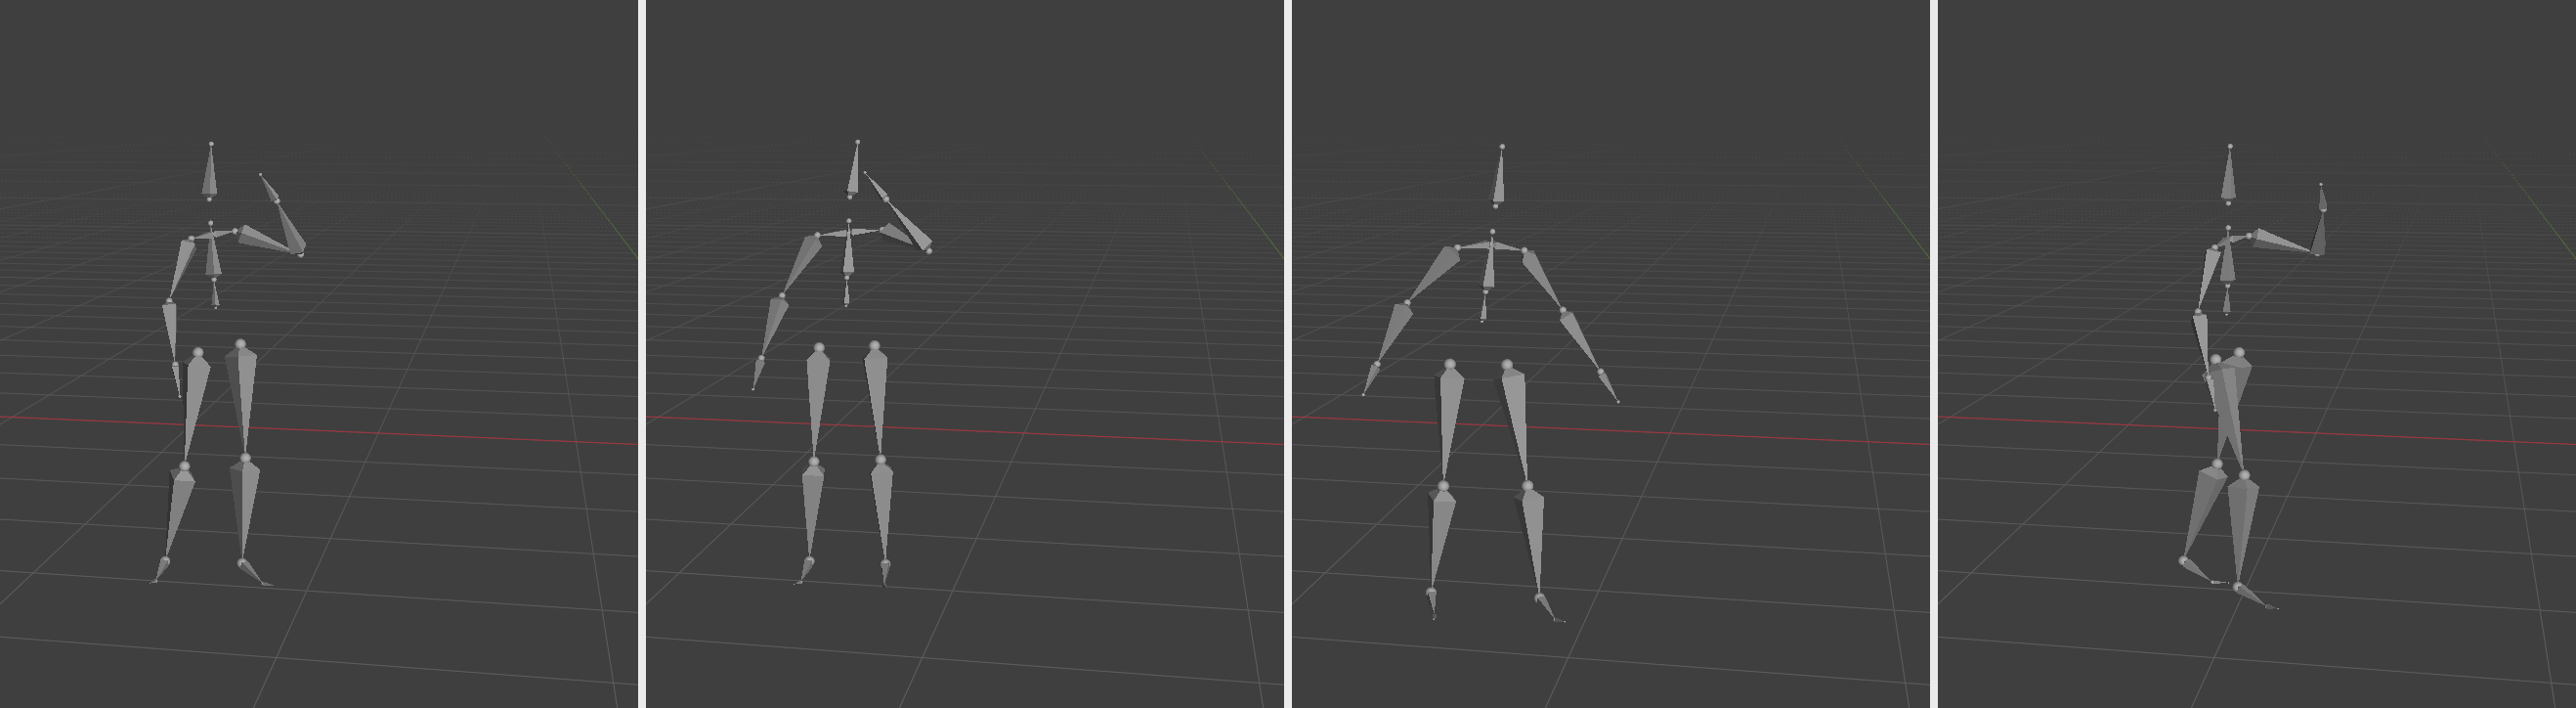
\includegraphics[width=\columnwidth]{fig_baseline.png}
\caption{Reproduced T2M-MoConGPT baseline: frames from a physically simulated
motion generated from a text prompt. The output is stylistically neutral,
motivating emotion conditioning.}
\label{fig:baseline}
\end{figure}

\subsection{Emotion Dataset Curation}
The keyword filter was applied to the 23{,}384 sequences (69{,}896 captions)
of the HumanML3D training split, yielding \textbf{463} emotion-labelled
caption--motion pairs (69{,}431 neutral, 2 conflicts discarded). The class
distribution is shown in Figure~\ref{fig:emodist}. Three findings emerge and
directly inform the plan:
\begin{itemize}
\item The yield (463) is \emph{below} the proposal's expected 800--1200:
HumanML3D captions are predominantly literal action descriptions and rarely
contain affective words.
\item The classes are strongly imbalanced (\textit{sad} has only 28 pairs),
which triggers the proposal's backup plan (class reduction, augmentation, and
the CMU emotional-gait supplement).
\item HumanML3D already ships left/right-mirrored copies; 229 of 463 pairs are
mirrors. Thus the proposed mirroring augmentation is effectively built in, and
the remaining lever is temporal speed augmentation ($0.8\times/1.2\times$,
$\approx\!3\times$ expansion).
\end{itemize}

\begin{figure}[t]
\centering
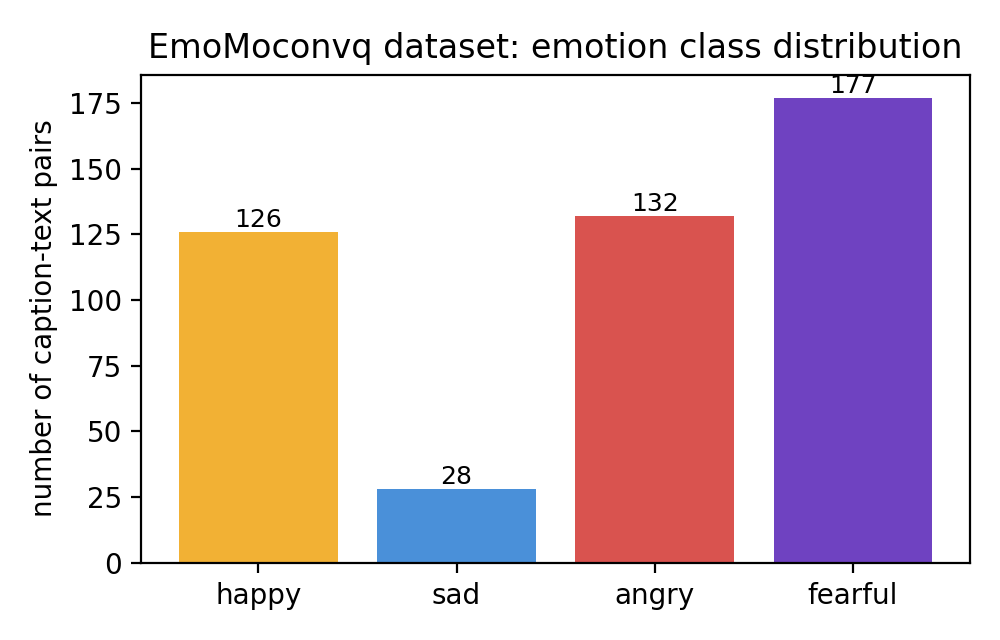
\includegraphics[width=0.86\columnwidth]{fig_emotion_dist.png}
\caption{Emotion class distribution of the 463 caption--motion pairs filtered
from the HumanML3D training split.}
\label{fig:emodist}
\end{figure}

\subsection{Emotion Module Verification}
The emotion module was validated by five structural checks
(Table~\ref{tab:verify}). Loading the pretrained checkpoint into
\texttt{EmoText2Motion\_Transformer} with \texttt{strict=False} leaves exactly
the 5 new emotion tensors uninitialized and produces \emph{no} unexpected
keys, confirming the module is a clean parameter superset of the baseline.
With the zero-initialization, the temporal feature with and without an emotion
label is bit-identical at step~0 (max difference $0.0$), verifying graceful
degradation; after perturbing the projection, \textit{happy} and \textit{sad}
produce clearly different outputs (max difference $1.40$), confirming the
conditioning pathway is functional. The configuration is parameter-efficient:
the emotion module is only $0.79$M parameters, and the full trainable set is
$47.3$M of $194.4$M ($24.3\%$).

\begin{table}[t]
\caption{Emotion module verification and parameter budget.}
\label{tab:verify}
\centering
\small
\begin{tabular}{lr}
\toprule
\textbf{Check / Quantity} & \textbf{Result} \\
\midrule
Missing emotion tensors on checkpoint load & 5 \\
Missing non-emotion tensors / unexpected keys & 0 / 0 \\
$|$out$(\varnothing)-$out(happy)$|$ at init (zero-init) & $0.0$ \\
$|$out(happy)$-$out(sad)$|$ after perturbation & $1.40$ \\
\midrule
Emotion module parameters & $0.79$M \\
Trainable parameters (emotion $+$ top-4 layers) & $47.3$M \\
Total model parameters & $194.4$M \\
Trainable fraction & $24.3\%$ \\
\bottomrule
\end{tabular}
\end{table}

\subsection{Initial Fine-Tuning}
Because the HumanML3D motions are SMPL-based kinematic vectors while the
MoConVQ encoder consumes physics-character observations, the labelled corpus
above does not yet carry MoConVQ motion tokens (see
Section~\ref{sec:remaining}). To still validate the fine-tuning pipeline
end-to-end, we ran a \emph{controlled overfitting experiment}: the one
MoConVQ-format motion shipped with the pretrained data (a CMU walking clip,
5227 frames) was encoded into RVQ tokens ($8\times1306$), sliced into five
50-step clips, and each clip was paired with an emotion-labelled caption. The
emotion-conditioned model was then fine-tuned with the NLL loss of
Eq.~\ref{eq:nll} for 60 steps.

Figure~\ref{fig:loss} shows the NLL dropping from $6.95$ to $\sim\!10^{-4}$,
while the emotion-module gradient norm is large early and decays as the model
converges -- the emotion module is genuinely trained (its embedding table
moves by $L_2=0.076$). An \emph{emotion-swap} diagnostic
(Table~\ref{tab:swap}) re-evaluates each clip with a wrong emotion label:
2 of 5 clips (\textit{neutral}, \textit{happy}) show a clear loss increase,
confirming the model does route information through the emotion signal; the
other 3 do not, because the teacher-forced latents alone already suffice for
those clips. This is an honest, expected outcome of a tiny controlled set:
it validates that \textbf{the fine-tuning loop and the emotion module are
correct and trainable}, while a genuine test of emotion controllability
requires the full dataset.

\begin{figure}[t]
\centering
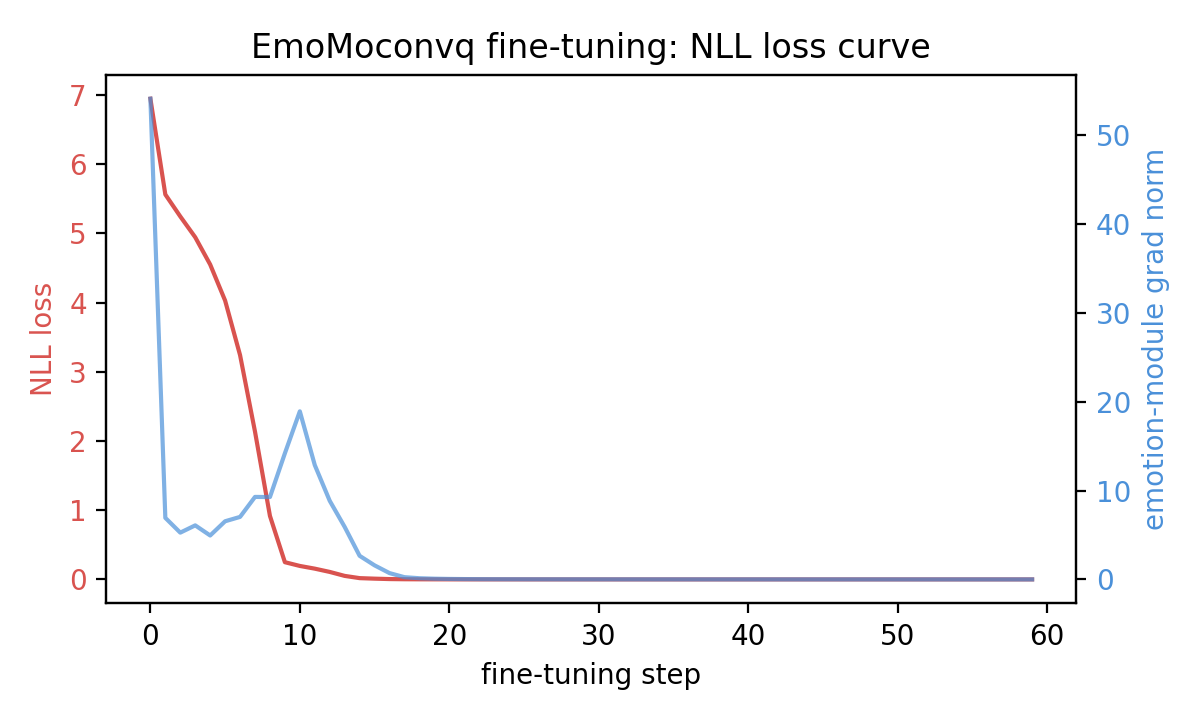
\includegraphics[width=\columnwidth]{fig_loss_curve.png}
\caption{EmoMoconvq fine-tuning. NLL loss (red) and emotion-module gradient
norm (blue) over fine-tuning steps in the controlled overfitting experiment.}
\label{fig:loss}
\end{figure}

\begin{table}[t]
\caption{Emotion-swap diagnostic: NLL with the correct vs.\ a wrong emotion
label after fine-tuning (lower is a better fit).}
\label{tab:swap}
\centering
\small
\begin{tabular}{lcc}
\toprule
\textbf{Clip} & \textbf{Correct label} & \textbf{Wrong label} \\
\midrule
neutral & $0.0001$ & $1.338$ \\
happy   & $0.0001$ & $0.174$ \\
sad     & $0.0001$ & $0.002$ \\
angry   & $0.0001$ & $0.000$ \\
fearful & $0.0001$ & $0.000$ \\
\midrule
mean    & $0.0001$ & $0.303$ \\
\bottomrule
\end{tabular}
\end{table}

\section{Remaining Work and Updated Plan}
\label{sec:remaining}
The experiments above place the project clearly past the proposal stage: the
baseline, the dataset pipeline, the emotion module, and the fine-tuning loop
are all implemented and verified. The main remaining work is:

\textbf{(1) Motion-tokenization pipeline.} The key gap is bringing HumanML3D
motions into MoConVQ's token space. HumanML3D motions are SMPL-based 263-d
kinematic vectors, whereas the MoConVQ encoder consumes physics-character
observations. We will build a retargeting path (HumanML3D/AMASS $\rightarrow$
BVH $\rightarrow$ MoConVQ character via the existing tracking utility),
producing the $(\text{text},\text{emotion},\text{tokens})$ triples needed for
real fine-tuning.

\textbf{(2) Full-scale fine-tuning} on the 463-pair set with temporal-speed
augmentation, supplemented by CMU emotional-gait clips for under-represented
classes (especially \textit{sad}); fall back to 3 classes if overfitting
occurs.

\textbf{(3) Quantitative evaluation:} FID, R-precision, an emotion-classifier
accuracy metric, and a small user study, as specified in the proposal.

Two practical issues were also resolved: a GPU-architecture mismatch (the
RTX~50-series is not natively supported by the available PyTorch build, which
falls back to PTX JIT) and the absence of public MoConGPT training code (the
loop was reimplemented). The updated timeline is given in
Table~\ref{tab:timeline}.

\begin{table}[t]
\caption{Updated project timeline. Tasks above the line are complete.}
\label{tab:timeline}
\centering
\small
\begin{tabular}{p{1.6cm}p{5.6cm}}
\toprule
\textbf{Status} & \textbf{Milestone} \\
\midrule
Done & Baseline reproduced; environment verified. \\
Done & Emotion dataset curated; statistics analysed. \\
Done & Emotion module implemented and verified. \\
Done & NLL fine-tuning loop implemented and validated. \\
\midrule
Next & Build HumanML3D$\rightarrow$MoConVQ tokenization. \\
Next & Full-scale emotion fine-tuning $+$ augmentation. \\
Next & Quantitative evaluation and user study. \\
Final & Report and demonstration video. \\
\bottomrule
\end{tabular}
\end{table}

\section*{Reproducibility and Attribution}
This project extends the pretrained MoConVQ~\cite{yao2023moconvq} framework.
All EmoMoconvq code -- the emotion module, the dataset filter, the
tokenization script, and the fine-tuning loop -- is original and contained in
new files; the upstream MoConVQ source is unmodified. Pretrained weights and
the HumanML3D~\cite{guo2022generating} annotations are used under their
respective terms.

\bibliographystyle{plainnat}
\bibliography{references}

\end{document}
